\documentclass[12pt]{chmullighw}
\usepackage{tikz}
\usepackage{tikz-qtree}
\usepackage{algorithm2e}
\usetikzlibrary{shapes}


% info for header block in upper right hand corner
\name{Chris Mulligan}
\uni{clm2186}
\class{COMS3137 Data Structures \& Algorithms}
\professor{Hershkop}
\assignment{Theory 2}
\duedate{October 20, 2013}

\lstset{language=Java, numbers=none, frame=l, captionpos=n}
\begin{document}
\problemlist{Theory 2} %Give us a nice big title
\begin{enumerate}

\item There is little advantage to an 8 item Linked List node, unless you can
make very strong assumptions regarding the contents of the Linked List. The
advantages include reduced memory allocations, which can be quite slow, and
an ability to proceed through a list in units of 8, particularly if you're able
to ignore the contents of the array inside each node.

The disadvantages include substantially increased complexity, an inability to
trivially rearrange the linked list, and potentially wasted space. It only seems
to make sense if you always have sets of 8, in which case it's really a normal
Linked List with each object being an 8-tuple.

Inserting a single element would be relatively easy, you would find the tail,
see if it has any space in the current LinkedNode8, and either add the element
to the end of the array if there's space, or allocate a new LinkedNode8 and 
insert into the beginning of the data array if not. This would be a simple \BigO{1}
operation, assuming we have a pointer to the tail.

Finding an element would be similar to a normal linked list find, with the added
complexity of checking all 8 spots in the arrays. You would start with head, check
all 8 spots, then proceed to the next node where you check all 8 nodes, and so on
until you reach the end or you find the element you're looking for. The result is
a standard \BigO{n} linear search.

Deleting an element is more complicated (I will assume we must preserve order,
since that's a feature of linked lists). First you have to do a find at \BigO{n}.
Then it depends on how you handle deletes. Option 1 would be to just empty the
array spot and shift all elements of the array left. This would leave the array
partially fully, but would guarantee all the empty spots are at the end of the
individual arrays to simplify things somewhat. While this means we can't guarantee
the node has 8 items, because the tail will often not have 8 items our code will
already have to accommodate that case so it should be relatively simple. Then if
the array is now entirely empty you could delete the node by pointing its previous 
to its next, and its next to its previous. This is \BigO{n} for the find, and
\BigO{1} for the delete, shift, and possibly deleting the node, for an overall of
\BigO{n}.

Similar would be to do lazy deletions of elements in a node, and only
delete the entire node when all elements have been lazily deleted. This would
add yet another level of complexity, for little benefit, so I would recommend
just leaving empty spots at the end of the array for the small additional fixed
cost of shifting up to 7 elements.

Deletion option 2 would be to compact the entire linked list, which would be much
more expensive. First a \BigO{n} find. Then we'd need to delete the element, and
shift all elements left in the node. Then we'd have to pop the first element from
the next node into the last slot of this node, then proceed through the rest of
the nodes shifting elements to the left, and taking the first from the next to be
the last for the current. Only at the end if the tail has a single element would we
delete the actual node. This would be \BigO{n} for the find, plus \BigO{n} for the
delete, for an overall run time of \BigO{n}, albeit with a larger constant than
option 1. 

So overall the big-O class of the 8 element linked list isn't particularly worse,
but code is more complicated and the constants are higher.


\item 
Output:
\begin{verbatim}
28  #Stack: [15]
81  #Stack: [15, 3]
3   #Stack: [15]
1   #Stack: [15, 9]
4   #Stack: [15, 9, 7]
7   #Stack: [15, 9]
4   #Stack: [15, 9]
\end{verbatim}

Final Stack: [15, 9]


\item \begin{enumerate} \renewcommand{\labelenumii}{\arabic{enumii}.}
\item \begin{enumerate} \renewcommand{\labelenumiii}{\arabic{enumiii}.}
\item The advantage to lazy deletion for arrays is that you can avoid frequently
compacting the array by shifting elements left by one, and more occasionally
compact the array by several. Compacting by any number of spaces requires
approximately the same amount of work, \BigO{n}, so if you can avoid doing 4
separate \BigO{n} shifts, and instead do a single one, you've reduced your runtime
from $4n$ to $n$.

The biggest disadvantage is that you make the code more complicated, as it must
now handle cases where elements have been deleted but remain in the list. It may
change the meaning of getting the $k^{th}$ value, or require substantially
increased runtime to determine which element actually is in position k. It can 
also slightly increase the amount of time required to find an element by value, since it has to skip over some elements.

Fortunately it doesn't require more memory, since the array has a fixed size,
and we can always decide to compact before we grow (although I imagine growing
and only copying alive values is more efficient for most uses). 

\item For a standard linked list there are no advantages to lazy deletion. Instead
of the standard \BigO{n} find plus \BigO{1} deletion after you find the element,
you have the \BigO{n} find, \BigO{1} to mark the element as deleted. Then at
some point another, separate \BigO{n} sweep to compact the list is required.

Moreover it wastes a lot more memory, since in a standard linked list we can
delete the node and immediately free the memory, with lazy deletion the node
stays around, using memory.

The one case it might make sense is if you were keeping an internal counter of
elements, and if you keep an element with a count of 0 around for a little while,
then if you re-add that element it will be faster to increment 0 than to create a
new node. However this case would be relatively rare for most use cases.
\end{enumerate}

\item In a standard binary tree this will cause extra work, and the tree
to be larger. That means the constants in the \BigO{\log n} runtime of operations
will be larger, and the overall tree will be slower.

In a binary search tree one advantage is that the tree will be reshuffled by
small amounts less, which could result in more balanced trees than naively deleting
as it occurs. Similarly in a self balancing tree, like AVL, you could do
fewer rotations, which could save some time. However it would mean that your tree
is larger, and therefore deeper for the same number of alive elements, slowing down operations.

Overall this mostly makes the trees more complicated, for little gain. 
\end{enumerate}

\item Let $l$ be the number of leaves, $n$ the total number of nodes, and $n_2$
as the number of nodes of degree 2. Every node has exactly 1 parent, except the
root. We shall prove $n_2 = l - 1$.

If $n = 1$ we only have a root, which is a leaf. $l$ = 1, $n_2$ = 0. \checkmark

Adding a node to a tree already displaying exhibiting this property, there are two cases:
\begin{itemize}
\item If it's the first child of a former leaf, we add increment $l$ for the new
node, but decrement $l$ because the former leaf is now degree 1. The degree of the grandparent, and all other nodes, is unchanged, so $n_2$ is unchanged. $l +1 -1 = l$, $n_2\prime = n_2$
\checkmark
\item If it's the second child of a former leaf, then both $n_2$ and $l$ are
incremented by one, and since $n_2 = l -1$ adding 1 to each side, $n_2 + 1 = (l + 1) - 1$, the equality still holds. \checkmark
\end{itemize}


\item
\tikzset{sibling distance=18pt}

a) \Tree[.18 ]
\hskip .8in
b) \Tree[.18   [.3 ]   \edge[draw=none];[.{} ] ]
\hskip .8in
c) \Tree[.18   [.3 ]
            [.25 ] ]
\hskip .8in
d) \Tree[.18   [.3 [.0 ] \edge[draw=none];[.{} ] ]
                [.25 ] ]

f) \Tree[.18   [.3 [.0 ] \edge[draw=none];[.{} ] ]
                [.25 \edge[draw=none];[.{} ] [.222 ] ] ]
\hskip 1.5in
g) \Tree[.18   [.3
                    [.0 \edge[draw=none];[.{} ] [.2 ] ]
                    \edge[draw=none];[.{} ] ]
                [.25 \edge[draw=none];[.{} ] [.222 ] ] ]

\-\\

h) \Tree[.18   [.3
                    [.0 \edge[draw=none];[.{} ] [.2 ] ]
                    [.11 ] ]
                [.25 \edge[draw=none];[.{} ] [.222 ] ] ]
\hskip 1in
i) \Tree[.18  [.3
                    [.0 \edge[draw=none];[.{} ] [.2 ] ]
                    [.11 \edge[draw=none];[.{} ] [.12 ] ] ]
                [.25 \edge[draw=none];[.{} ] [.222 ] ] ]

\-\\

j) \Tree[.18  [.3
                    [.0 \edge[draw=none];[.{} ] [.2 ] ]
                    [.11 \edge[draw=none];[.{} ] [.12 ] ] ]
                [.25
                    \edge[draw=none];[.{} ]
                    [.222 [.34 ] \edge[draw=none];[.{} ] ] ] ]
\hskip .5in
k) \Tree[.18  [.3
                    [.0 \edge[draw=none];[.{} ] [.2 ] ]
                    [.11 \edge[draw=none];[.{} ] [.12 ] ] ]
                [.25
                    \edge[draw=none];[.{} ]
                    [.222
                        [.34 [.30 ] \edge[draw=none];[.{} ] ]
                        \edge[draw=none];[.{} ] ] ] ]

\-\\

l) Final: \Tree[.18  [.3
                    [.0 \edge[draw=none];[.{} ] [.2 ] ]
                    [.11 \edge[draw=none];[.{} ] [.12 ] ] ]
                [.25
                    \edge[draw=none];[.{} ]
                    [.222
                        [.34 [.30 ] [.40 ] ]
                        \edge[draw=none];[.{} ] ] ] ]

\-\\

Pre-Order: 18, 3, 0, 2, 11, 12, 25, 222, 34, 30, 40

Post-Order: 2, 0, 12, 11, 3, 30, 40, 34, 222, 25, 18

In-order: 0, 2, 3, 11, 12, 18, 25, 30, 34, 40, 222

\item First, set the root node's depth to 0. For each node set their children's
depth to the node's depth + 1. Then recursively call the same routine on each of
the children.

This is \BigO{n} because every node is touched once when its depth is updated,
and once to get all its children. With clever programming that could be reduced
to only once, but both cases are \BigO{n}.

\item  \hskip 1in

\begin{algorithm}[H]
\SetAlgoNoLine
\KwData{Tree T}
\KwResult{A \BigO{n} algorithm for non-recursively in-order traversing a binary tree.}

create stack\;
current = root\;
\While{current is not null or stack is not empty}{
    \If(\tcc*[h]{pop from the stack, and head right}){current is null}{
        current = stack.pop\;
        process current\;
        current = current.right\;
    }
    \If(\tcc*[h]{push onto stack and proceed left}){current is not null}{
        push current onto stack\;
        current = current.left\;
    }
}
\end{algorithm}

This algorithm is \BigO{n} because each node is only touched twice, once when
it is pushed onto the stack, and once when it's popped off and processed. 

\item 
Initial: 
\Tree[.14   [.4 [.2 ] [.13 ]  ]
            [.15 \edge[draw=none];[.{} ] [.18 [.17 ] [.39 ]]]]

After deleting the root (14), we move smallest on right to root:\\
\Tree[.15   [.4 [.2 ] [.13 ]  ]
            [.18 [.17 ] [.39 ]]]

\item After inserting 2, 1, 4, 5, 9, 10, 11:\\
\Tree[.5  [.2  [.1 ]  [.4 ] ]
          [.10  [.9 ]  [.11 ] ] ]

After inserting 13, 3, 17, 33:\\
\Tree[.5 [.2  [.1 ]
              [.4  [.3  ] \edge[draw=none];[.{} ]  ] ]
  [.13  [.10  [.9 ] [.11 ] ]
        [.17  \edge[draw=none];[.{} ]  [.33 ]  ] ] ]

\newpage
\item B+Tree with M=5, L=7, after inserting: 4, 40, 23, 50, 11, 34, 62, 78, 66, 22, 90, 59, 25, 72, 64, 77, 10, 12.

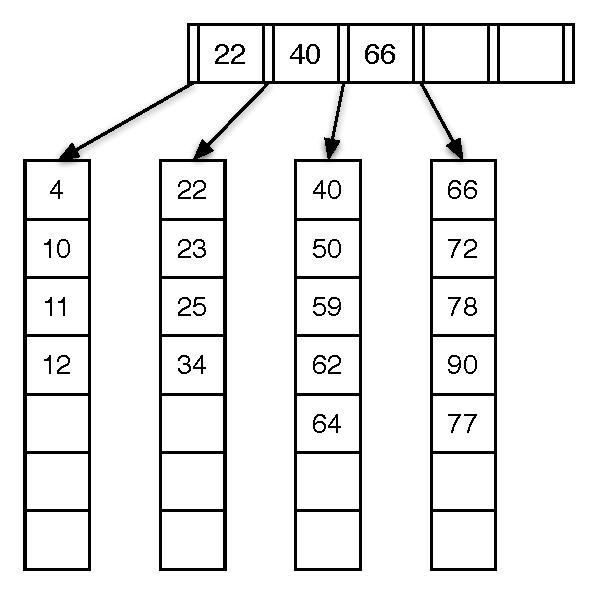
\includegraphics{q10.pdf}

\newpage
\item This algorithm will work, called with isSimilar on the root nodes. 

\begin{algorithm}[H]
\SetAlgoNoLine
\KwData{Tree a, Tree b}
\KwResult{Recursively determine if two binary trees have the same shape}
\SetKwProg{Fn}{Function}{ is}{end}

\Fn{isSimilar(node a, node b)}{
    \uIf{a is null and b is null}{
        return true\;
    }
    \uElseIf{a is null and b is not null}{
        return false\;
    }
    \uElseIf{a is not null and b is null}{
        return false\;
    }
    \Else{
        leftSimilar = isSimilar(a.left, b.left)\;
        rightSimilar = isSimilar(a.right, b.right)\;
        return (leftSimilar and rightSimilar)\;
    }
}
\end{algorithm}

The runtime is \BigO{n}, where n is the size of the smaller tree. It must touch
every element in both trees to verify they're equal, hence \BigO{n}.

\item AVL and Splay trees are both binary search trees that use auto balancing to
prevent degenerate cases of unbalanced trees. They go about it in different ways.

In an AVL tree the tree is balanced whenever a node is inserted or deleted. It
ensures that along the entire insert path no nodes left and right sides have
heights that differ by more than 1. If they do it performs rotations, either single
or double, to bring the tree back into balance. Thus after every insert and delete
it guarantees the left and right sides of every node will have similar heights.
Insert, find, and delete are all \BigO{\log n}. 

A splay tree uses similar rotations, called zig-zigs and zig-zags, to balance the
tree. However splay trees balances on finds, rather than on inserts. Whenever a
node is found, it is rotated to be the root node. By rotating along the way the
tree comes closer into balance. This permits the tree to be quite unbalanced
(even becoming a linked list in the worst case), but for a sequence of finds
and inserts the tree performs with an amortized \BigO{\log n} runtime. In other
words, for any $M$ operations the runtime is \BigO{M\log n}

AVL trees guarantee that the height of the tree is always approximately $\log n$,
however inserts can be slower, and they don't further optimize. Splay trees may
have cases with very large heights, but they guarantee that more recently accessed
nodes are near the top, which helps with real world usage. Further, splay trees
ensure that the overall runtime is no worse than AVL for a large sequence of
operations.

\end{enumerate} %end of questions
\end{document}
